% Question  ##################################################################################################################
\section{Question 2}\label{ssec:pt2q2}
\textbf{In this question we will analyse Apple Stock.}
% END Question  ##############################################################################################################

% Question (i) ###############################################################################################################
\subsection{Q2 (i)}\label{sssec:pt2q2i}

\textbf{Download closing prices for Apple for the period 01/01/2013 and 30/11/2017. Apply daily log returns and measure the average daily return.}

\noindent
Code to download the closing prices for Apple can be found in ‘Question 2 (i)’ in the python notebook. The data was downloaded from Yahoo Finance and saved as .csv format in the following path \textit{‘src/data/part\_2’}. The file was saved as \textit{‘AAPL.csv’}. The data was then reloaded from the file and converted into pandas dataframe.

\noindent
After applying the log returns the measure of the average daily log returns was 0.091\%.

% END Question (i) ###########################################################################################################

% Question (ii) ##############################################################################################################

\subsection{Q2 (ii)}\label{sssec:pt2q2ii}
\textbf{We wish to measure volatility. Compare and discuss pros and cons of utilising the Historical method, Exponentially Moving Average method or Garch.}

\noindent
\textit{Historical Method}

\noindent
To measure volatility using the historical method, first the historic data must be obtained. Once the data is obtained the log returns must be calculated and then the standard deviation is calculated on the log returns. In this model when higher frequency data is used the sum of the squared returns is used instead. In this method all past data is given an equal weight (no weight at all). 

Pros:
\begin{itemize}
    \item Faster to compute and easy to implement. 
    \item Does not require any parameters.
    \item No model risk since no parameters are used.
\end{itemize}

Cons:
\begin{itemize}
    \item Does not assign any weights and all values are given the same importance.
    \item Less accurate since it does not give importance to recent values. 
    \item Data is not utilised properly (most of the data is not used). 
\end{itemize}

\noindent
\textit{EWMA}

\noindent
Unlike the historical method, the exponentially weighted moving average method does not give equal weights to the data points.  This is done as the recent square returns should give a better indication for volatility. In this method an exponentially decreasing weight is set to the squared returns (starts from the most recent data point).

Pros:
\begin{itemize}
  \item Assigns exponentially decreasing weight to the squared returns. Recent returns better describe volatility. 
  \item Less parameters than the GARCH model, thus less Model Risk.
\end{itemize}

Cons:
\begin{itemize}
    \item This model do not handle mean reversion (no term used for mean reversion). 
    \item Does not capture trend information.
    \item Does not forecast volatility. 
    \item A volatility shock is suddenly dropped from the computation as the trailing window of observations pass. 
\end{itemize}

\noindent
\textit{Garch}

\noindent
The Generalized ARCH model is an extension to the ARCH model. This model also uses weights, but the weights are assigned to the following three components; lagged variance, lagged squared return and the long-run variance. The sum of the weights assigned to the first two components is known as persistence. Commonly this model is solved using the maximum likelihood estimation technique.

Pros:
\begin{itemize}
  \item More weight on recent information.
  \item Can output more accurate estimations. 
  \item A term is used to handle mean reversion. 
  \item Can be used to forecast volatility. 
  \item Overcomes Ghosting as a shock in volatility will be immediately impact the estimates (Fades as time passes).
\end{itemize}

Cons:
\begin{itemize}
    \item This models requires more parameters and has a greater Model Risk.
    \item More computationally expensive. 
\end{itemize}

\noindent
Comparing the three models, the first model does not assign weights to the log returns, while the EWMA uses exponentially decreasing weights to the squared returns. On the other hand, the GARCH models’ assigns weights to the following components lagged variance, lagged squared returns and long run variance. Both the GARCH and EWMA work with conditional variance but the other model works with realized variance. Also both GARCH and EWMA apply exponential smoothing to their weights. Unlike GARCH the EWMA does not have a term for mean reversion. Both GARCH and EWMA are recursive and parametric. 


% END Question (ii) ##########################################################################################################

% Question (iii) #############################################################################################################

\subsection{Q2 (iii)}\label{sssec:pt2q2iii}
\textbf{Use Garch(1,1) to measure volatility based on the data from (i).}

\noindent
The measurement for the annualized volatility for Apple when using Garch(1,1) is 22.46\%. 

\noindent
Volatility was computed using the code found in ‘Question 2 (iii)’ in the python notebook and this notebook cell utilises a function called 'arch\_vol' found in the 'fintech' library. Such function uses a third party library called 'arch' \cite{python:arch} which provides different volatility models written in python. 

% END Question (iii) #########################################################################################################

% Question (iv) ##############################################################################################################

\subsection{Q2 (iv)}\label{sssec:pt2q2iv}
\textbf{Assume that Apple stock prices follow a Geometric Brownian stochastic process. Utilising the average return and volatility statistics identified in part (i) and (iii), simulate, on a day by day basis, the movement of Apple stock for the next 20 days (i.e. starting from 1st December, as per date range in part (i)). Repeat this process for 100 times, hence creating 100 possible price realisations over the next 20 days. Describe the steps/approach used and present a plot showing the projected 100 realisations.}

\noindent
First the current price was referenced, which is the adjusted close price for the 1st of December. The expected volatility was computed by using the annualized volatility found in (iii) and scaling it to get the expected volatility for the next day. This was done using the following computation (assuming a year has 250 days) $(Annualized \ Volatility \times \sqrt{\frac{1}{250}})$. 

\noindent
Now that we have the expected return and expected volatility, an iteration to create different projections was written. The iteration runs for 100 times, since we need to create 100 possible price realisations. In each iteration a new Brownian path is generated using a function which was created in the ‘fintech’ library called ‘brownian\_motion’ as shown in Fig.~\ref{fig:brownpath}. When calling this function, the number of increments is passed as a parameter which in our case is 20 since we are projecting for the next 20 days. 

\begin{figure}[H]
\centering
  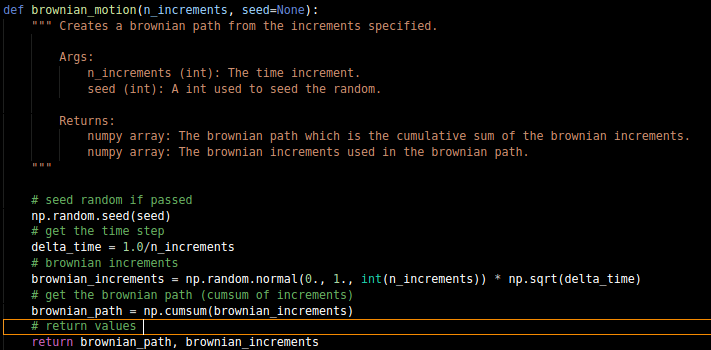
\includegraphics[scale = .64]{imgs/brownian_path.png}
  \caption{Function to create Brownian path.}
  \label{fig:brownpath}
\end{figure}

\noindent
In this function the Brownian increments $W_i$ are computed by getting $z_i$ which is a random variable selected from a normal distribution with $\mu=0$ and $\sigma=1$ and multiplying it by $\sqrt{t_i}$ where $t_i$ is the time increment, as shown in Eq.~\ref{eq:brownincr}.  

\begin{equation} \label{eq:brownincr}
    W_i = z_i \sqrt{\Delta t_i}
\end{equation}

\noindent
After computing the Brownian increments, the Brownian path is computed by getting the cumulative sum of the Brownian increments. This is shown in Eq.~\ref{eq:brownpath}, and the 'brownian\_motion' function returns both the path and the increments. 
 
\begin{equation} \label{eq:brownpath}
    W_n(t) = \sum_{i=1}^{n} W_i(t)
\end{equation}

\noindent
In each iteration when a new Brownian path is generated, the path is used as a parameter in a function called 'geo\_brownian\_motion' which is also found in the 'fintech' library and this function is shown in Fig.~\ref{fig:browngeo}. The returned stock prices and time periods were used to plot the possible price realisations. Each price at $t$ is computed using Eq.~\ref{eq:geobrown}. 

\begin{figure}[H]
\centering
  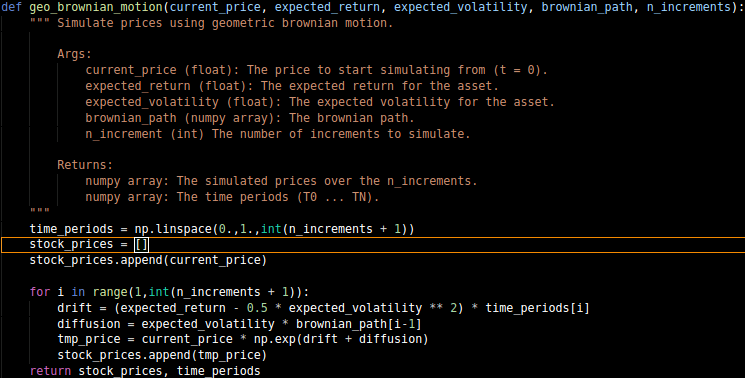
\includegraphics[scale = .64]{imgs/geo_brown_path.png}
  \caption{Function to create Geometric Brownian Motion.}
  \label{fig:browngeo}
\end{figure}

\begin{equation} \label{eq:geobrown}
    S_{t+\Delta t} = S_t \exp[(\mu - \frac{\sigma^2}{2}) + \Delta t + \sigma \epsilon \sqrt{\Delta t}] 
\end{equation}

\noindent
These functions were then called in the notebook in 'Question 2 (iv)' as shown in Fig.~\ref{fig:notebrown} and the final output was plotted as shown in Fig.\ref{fig:notebrownplot}.

\begin{figure}[H]
\centering
  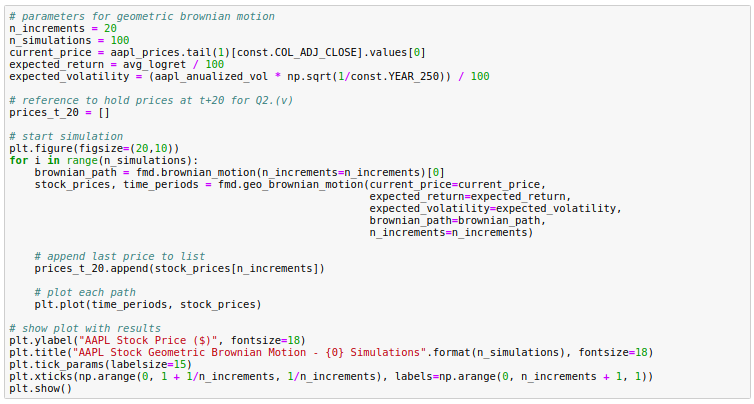
\includegraphics[scale = .60]{imgs/simulation100.png}
  \caption{Code for simulation using Geometric Brownian path.}
  \label{fig:notebrown}
\end{figure}

\begin{figure}[H]
\centering
  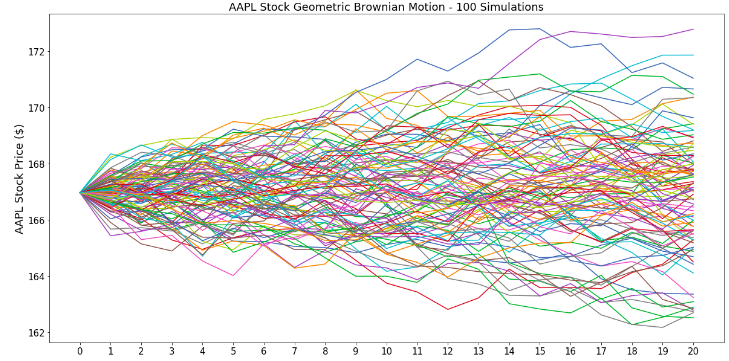
\includegraphics[scale = .64]{imgs/simulationplot.png}
  \caption{100 price realisations over the next 20 days using Geometric Brownian Motion.}
  \label{fig:notebrownplot}
\end{figure}

% END Question (iv) ##########################################################################################################

% Question (v) ###############################################################################################################

\subsection{Q2 (v)}\label{sssec:pt2q2v}
\textbf{Using the prices obtained at the end of each simulated realisation, i.e. simulated prices at
t+20 days, calculate the 20 day Value at Risk (VaR) at 95\% confidence level. Hint: You can
use the percentile approach on the 20 day returns. }

\noindent
The 20 day VaR(95\%) based on the simulation for question (iv) is \$3.40. Code for this measurement is shown in 'Question 2 (v)' in the notebook.

% END Question (v) ###########################################################################################################
